% Version 2.20 of 2017/10/04
%
\documentclass[runningheads]{llncs}
%

\usepackage{wrapfig,floatrow}

% used for FloatBarrier
\usepackage{placeins}

\usepackage{minted}

\usepackage{soul} % color, soul - required for text highlighting
\usepackage{xcolor} %% http://www.ctan.org/pkg/xcolor
\usepackage{graphicx}
% Used for displaying a sample figure. If possible, figure files should
% be included in EPS format.

\usepackage{hyperref}
% linkcolor=blue!50!red,
% \hypersetup{
%   colorlinks=true,
%   linkcolor=green!80,
%   urlcolor=blue
% }

% If you use the hyperref package, please uncomment the following line
% to display URLs in blue roman font according to Springer's eBook style:
% \renewcommand\UrlFont{\color{blue}\rmfamily}

\usepackage{bibnames}





\begin{document}
%
\title{PyFaaS - Towards a Scalable and Distributed Python Function-as-a-Service (FaaS)}
%
%\titlerunning{Abbreviated paper title}
% If the paper title is too long for the running head, you can set
% an abbreviated paper title here
%
\author{Dan Alexandru, Rares Dima, Matei Micu}
%
% \authorrunning{Dan Alexandru et al.}
% First names are abbreviated in the running head.
% If there are more than two authors, 'et al.' is used.
%
\institute{Department of Computer Science, “Al.I.Cuza” University of Iasi, Romania}
%
\maketitle              % typeset the header of the contribution
%
\begin{abstract}
In the current cloud landscape, we identified a particular need for a robust FaaS for Python that would aid both developers and researchers in their Python workflows. As such, we leverage existing cloud infrastructure to allow flexible workflows both over existing FaaS and IaaS solutions.

\keywords{Software Engineering \and Cloud Computing \and FaaS \and Function as a Service \and Python}
\end{abstract}
%
%%%%%%%%%%%%%%%%%%%%%%%%%%%%%%%%%%%%%%%%%%%%%%%%%%%%%%%%%%%%%%%%%%%%%%%%%%%%%%%%%%%%%%%%%%%
%

\section{Introduction}




% \smallskip\hrule\smallskip

\FloatBarrier
%%%%%%%%%%%%%%%%%%%%%%%%%%%%%%%%%%%%%%%%%%%%%%%%
\section{State of the art / Related work}

% \begin{itemize}
%   \item sentiment analysis \begin{itemize}
%     \item polarity
%   \end{itemize}
%   \item aspect-based sentiment analysis\begin{itemize}
%     \item polarity
%   \end{itemize}
% \end{itemize}

The current form of the Serverless Paradigm appeared in 2015, when cloud providers have identified the need for developers to have simpler solutions than IaaS, and more atomic than PaaS.

\begin{figure}
    \centering
    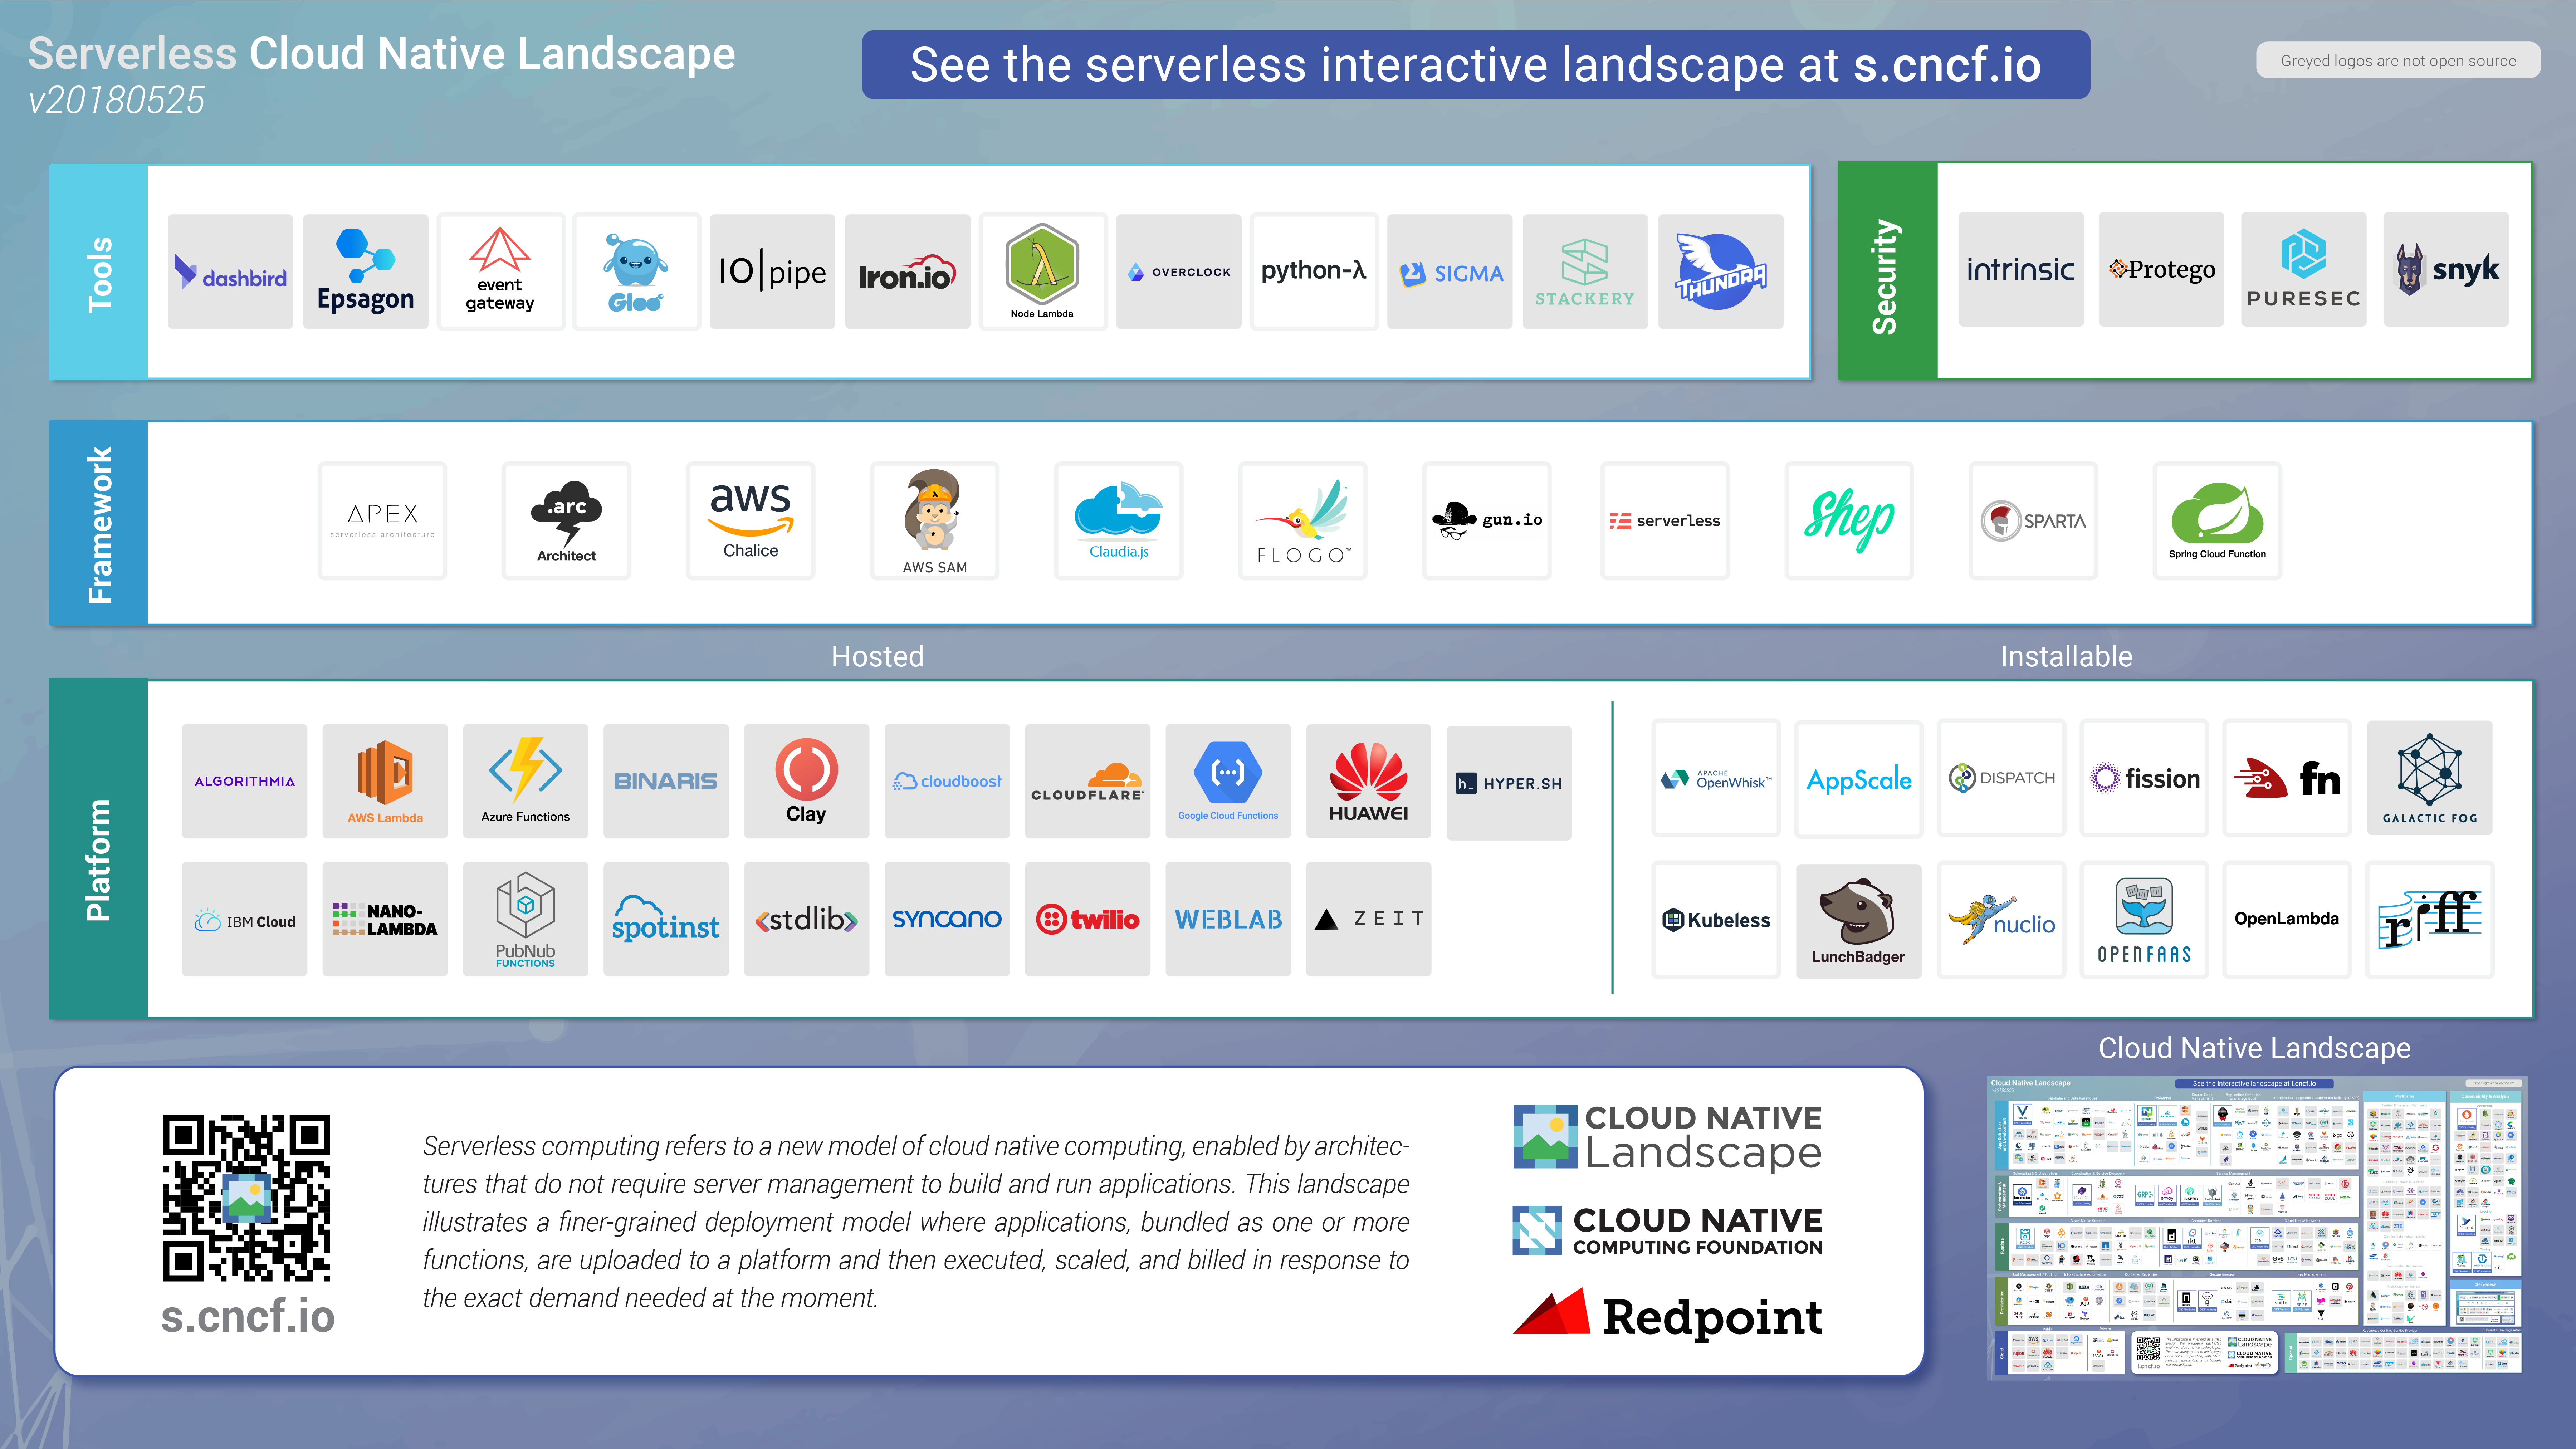
\includegraphics[scale=0.25]{assets/CNCF_landscape_min.png}
    \caption[SOTA-Landscape]{The current landscape of FaaS, as provided by Cloud Native Computing Foundation Serverless Working Group (\url{https://github.com/cncf/wg-serverless}). An Interactive version is provided at \url{https://s.cncf.io/}}.
    \label{fig:SOTA-Landscape}
\end{figure}

 As such, Amazon came with AWS Lambda, which enabled devices like Amazon Echo to call various functions.
 
 To avoid vendor lock-in, certain companies chose to make their own solution of FaaS that could be deployed over multiple cloud vendors' solutions, such as \url{https://github.com/serverless/serverless} or \url{https://github.com/iron-io/functions}.
 

% \hrule\smallskip
\FloatBarrier
%%%%%%%%%%%%%%%%%%%%%%%%%%%%%%%%%%%%%%%%%%%%%%%%
\section{Architecture}

% \begin{wrapfigure}{R}{0.4\textwidth}
%   \begin{center}
%     \includegraphics[scale=0.5]{methods-tree-01.jpg}
%   \caption[Memrise 1]{Memrise Home Page}
%   \label{fig:Memrise-1}
%   \end{center}
% \end{wrapfigure}

We propose a solution leaning towards a Service-Oriented Architecture (SOA). All components are atomic, containerized, easy to swap and to upgrade.

\begin{figure}
    \centering
    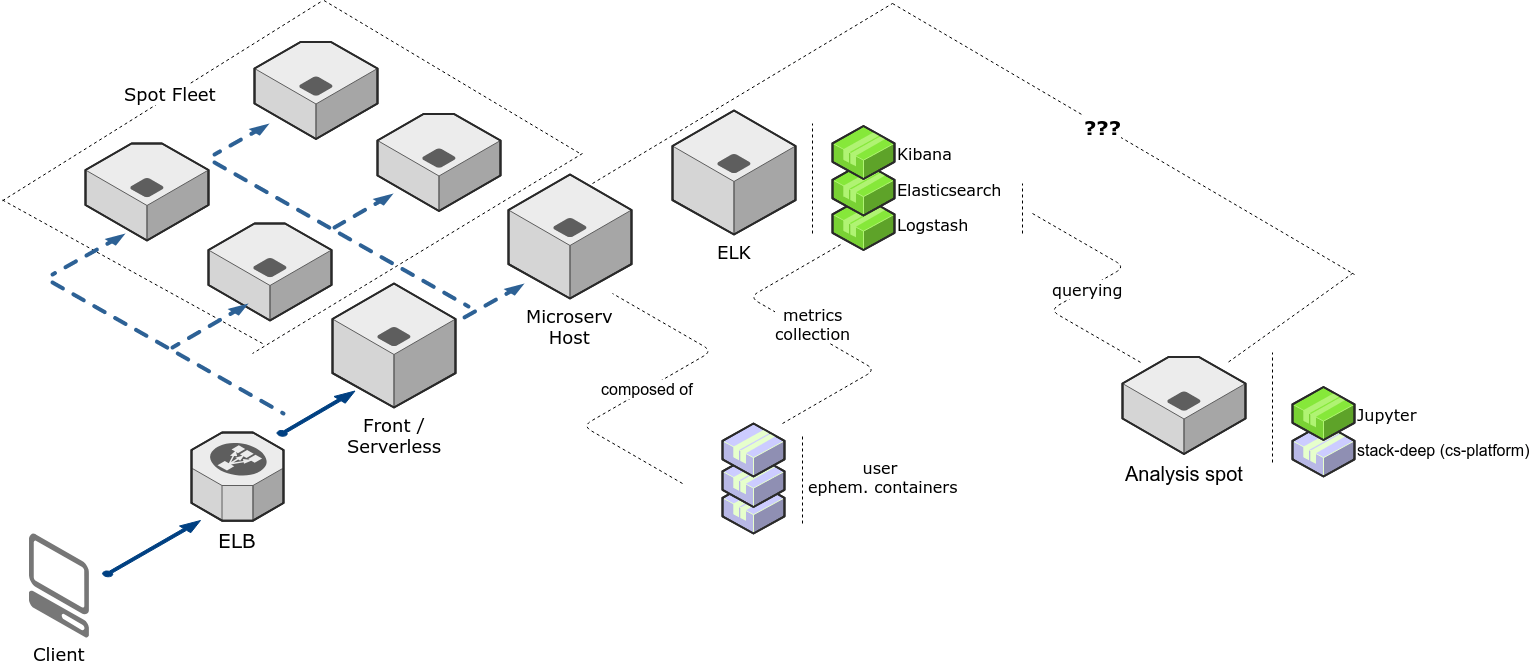
\includegraphics[scale=0.22]{assets/init_min.png}
    \caption[Architecture]{Our currently proposed architecture.}
    \label{fig:Architecture-01}
\end{figure}

As it is, a user would connect to a web application that provides the service where they could add or edit their function, afterwards running in a one or multiple hosts, during which logs will be displayed to the user.

The anoymized metadata from the ephemeral containers and the functions that are deployed is stored, queried and displayed in the ELK stack (Elasticsearch, Logstash, Kibana - Logstash stores, Elasticsearch indexes and exposes an API, Kibana displays metrics). Furthermore, Elasticsearch can be queried in analysis ephemeral instances (in AWS context - spot instances) which host an Python analysis container for easier visualization, and use of data. Eventually, that spot should offer the possibility to create metrics, alarms, automatically-updated notebooks or models.


\FloatBarrier
%%%%%%%%%%%%%%%%%%%%%%%%%%%%%%%%%%%%%%%%%%%%%%%%
\section{Load prediction}


Load balancing was a constant concern ever since the web started expanding. Too little compute power and a site becomes slow and unresponsive, losing users and thus revenue, too much and you’d be throwing money away, negatively impacting profit. 

This created the need for load balancing. However adding more compute power after the user’s performance has already been impacted, especially since adding more compute power is often not very fast, only leads to limited gains. In the current market, where employing machine learning techniques becomes more and more practical, it comes as a natural extension to load balancing: replacing reaction with proaction.

Due to the volatile nature of web traffic and lack of massive datasets, research in the field has been inconsistent, however, this exact advent has been growing more and more in the field of electrical load balancing \cite{He2017LoadFV}, for energy suppliers like E-ON. Research into using convolutional recurrent deep neural networks has yielded positive results in forecasting load on a ‘per week’ basis, forecasting loads for each day of the week.

For example higher loads in the middle of the day, lower loads during the nights when people usually sleep, and the same pattern during the weekends but with slightly elevated levels.


\begin{figure}
    \centering
    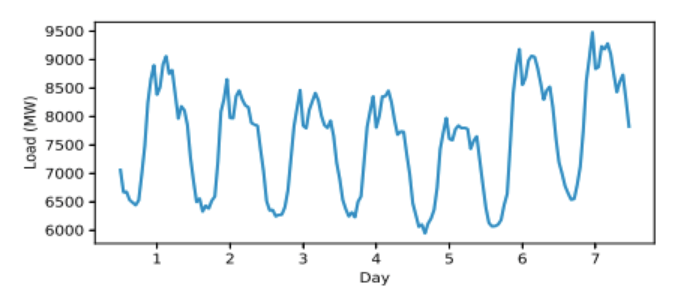
\includegraphics[scale=0.4]{assets/load-prediction-01_min.png}
    \caption[LoadPred]{How businesses such as electricity services predict usage during a day}
    \label{fig:LoadPrediction-01}
\end{figure}


Less prevalent, but still present, is an area of study somewhat more related to the present project: server load prediction. This field also has employed neural networks to achieve load prediction\cite{Aljabari2018}:


\begin{figure}
    \centering
    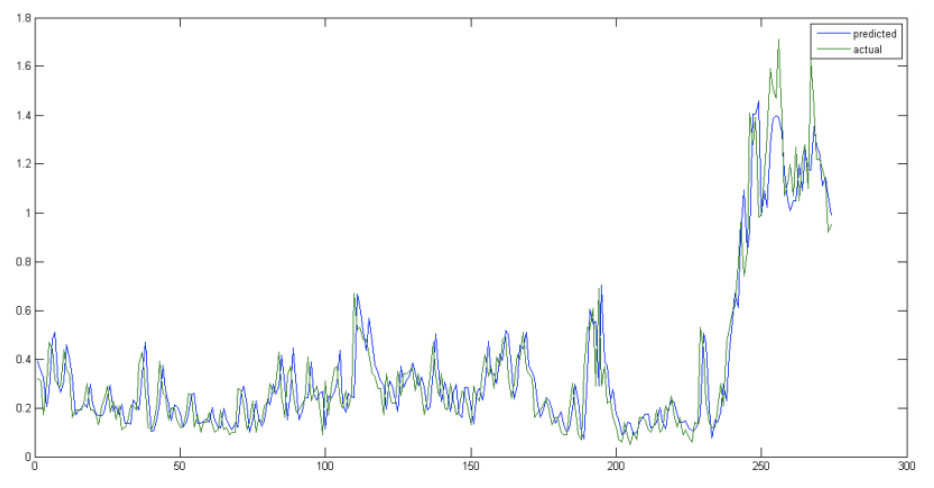
\includegraphics[scale=0.4]{assets/load-prediction-02_min.png}
    \caption[LoadPred]{How we perform load prediction on simulated data}
    \label{fig:LoadPrediction-02}
\end{figure}


Although this application is closer to the current scope, it is still something different as server load is a different matter from a theoretically infinite cluster of compute spots that can simply scale up power and cost until the stipulated demands are met. 

Nonetheless, the core of both of these project is achieving prediction on a time series, and while the applications of such an endeavour vary wildly, the core ideas of the field are completely portable.



\FloatBarrier
%%%%%%%%%%%%%%%%%%%%%%%%%%%%%%%%%%%%%%%%%%%%%%%%
\section{Conclusions}

...

% \hrule\smallskip
%%%%%%%%%%%%%%%%%%%%%%%%%%%%%%%%%%%%%%%%%%%%%%%%

 
\pagebreak

% Reviews - \cite{MantylaGK16}
% \noindent MS Theses - \cite{Park2018}


\bibliographystyle{splncs04}
\bibliography{resources}

%
%%%%%%%%%%%%%%%%%%%%%%%%%%%%%%%%%%%%%%%%%%%%%%%%%%%%%%%%%%%%%%%%%%%%%%%%%%%%%%%%%%%%%%%%%%%
%
% \section{First Section}
% \subsection{A Subsection Sample}
% Please note that the first paragraph of a section or subsection is
% not indented. The first paragraph that follows a table, figure,
% equation etc. does not need an indent, either.

% Subsequent paragraphs, however, are indented.

% \subsubsection{Sample Heading (Third Level)} Only two levels of
% headings should be numbered. Lower level headings remain unnumbered;
% they are formatted as run-in headings.

% \paragraph{Sample Heading (Fourth Level)}
% The contribution should contain no more than four levels of
% headings. Table~\ref{tab1} gives a summary of all heading levels.

% \begin{table}
% \caption{Table captions should be placed above the
% tables.}\label{tab1}
% \begin{tabular}{|l|l|l|}
% \hline
% Heading level &  Example & Font size and style\\
% \hline
% Title (centered) &  {\Large\bfseries Lecture Notes} & 14 point, bold\\
% 1st-level heading &  {\large\bfseries 1 Introduction} & 12 point, bold\\
% 2nd-level heading & {\bfseries 2.1 Printing Area} & 10 point, bold\\
% 3rd-level heading & {\bfseries Run-in Heading in Bold.} Text follows & 10 point, bold\\
% 4th-level heading & {\itshape Lowest Level Heading.} Text follows & 10 point, italic\\
% \hline
% \end{tabular}
% \end{table}


% \noindent Displayed equations are centered and set on a separate

% Please try to avoid rasterized images for line-art diagrams and
% schemas. Whenever possible, use vector graphics instead (see
% Fig.~\ref{fig1}).

% \begin{figure}
% \includegraphics[width=\textwidth]{fig1.eps}
% \caption{A figure caption is always placed below the illustration.
% Please note that short captions are centered, while long ones are
% justified by the macro package automatically.} \label{fig1}
% \end{figure}

% \begin{theorem}
% This is a sample theorem. The run-in heading is set in bold, while
% the following text appears in italics. Definitions, lemmas,
% propositions, and corollaries are styled the same way.
% \end{theorem}

%
% the environments 'definition', 'lemma', 'proposition', 'corollary',
% 'remark', and 'example' are defined in the LLNCS documentclass as well.
%

% \begin{proof}
% Proofs, examples, and remarks have the initial word in italics,
% while the following text appears in normal font.
% \end{proof}


%  an LNCS chapter~\cite{ref_lncs1}, 
% \cite{ref_lncs1,ref_url1}.
%
% ---- Bibliography ----
%
% BibTeX users should specify bibliography style 'splncs04'.
% References will then be sorted and formatted in the correct style.
%
% \bibliographystyle{splncs04}
% \bibliography{mybibliography}
%


% \begin{thebibliography}{8}

% \bibitem{ref_lncs1}
% Author, F., Author, S.: Title of a proceedings paper. In: Editor,
% F., Editor, S. (eds.) CONFERENCE 2016, LNCS, vol. 9999, pp. 1--13.
% Springer, Heidelberg (2016). \doi{10.10007/1234567890}

% \bibitem{ref_url1}
% LNCS Homepage, \url{http://www.springer.com/lncs}. Last accessed 4
% Oct 2017

% \end{thebibliography}




\end{document}
